\documentclass[a4paper]{article}

\usepackage[T1]{fontenc}
\usepackage[utf8]{inputenc}
\usepackage{graphicx}
\usepackage{color}
\usepackage[intlimits]{amsmath}
\usepackage{amsfonts}
\usepackage{listings}
\usepackage{float}
\usepackage{setspace}
\usepackage{english,babel}
\usepackage{fancyhdr}
\usepackage{booktabs}
\usepackage{multirow}
\usepackage{lastpage}
\usepackage[arrowmos]{circuitikz}
\usepackage[nottoc]{tocbibind}
\usepackage{url}
\usepackage[ugly]{units}
\usepackage[left=1.5cm,top=2cm,right=1.5cm,bottom=2.5cm]{geometry}
\usepackage[pdftex]{hyperref}
\usetikzlibrary{patterns,decorations.pathreplacing,automata,positioning,shapes,arrows}
\usepackage[T1]{fontenc}
%\usepackage{libertine}
\renewcommand*\oldstylenums[1]{{\fontfamily{fxlj}\selectfont #1}}
\setcounter{secnumdepth}{0}

\DeclareMathOperator{\ld}{ld}

\onehalfspacing
\setlength{\parindent}{0pt}

%\widowpenalty=1000
%\clubpenalty=1000

\tocsection

\author{Mathias Plichta}

\begin{document}
	\pdfinfo
	{/Creator (Mathias Plichta)
	 /Producer (pdflatex)
	 /Author (Mathias Plichta)
	}

\pagestyle{fancy}
\fancyhead{}
\fancyfoot{}
\renewcommand{\headrulewidth}{0pt}
\setlength{\parskip}{6pt}
\renewcommand{\headrulewidth}{.4pt}
\fancyhead[r]{Mathias Plichta, group 3}
\fancyhead[c]{Projektpraktikum IC-Entwurf}
\fancyhead[l]{Technische Universität München}
\fancyfoot[c]{Seite \thepage\ von \pageref{LastPage}}

\section{Display Driver}

\subsection{Overview}

The display driver translates character data into the signals required to
control the display. It also generates the sequence required to initialize the
display.

\begin{figure}
	\begin{center}
		\begin{tikzpicture}
			%\draw[help lines] (-2, -6) grid (4, 2);

			\node[above] at (3,0) {display\_driver};

			\draw[line width=2pt,->] (-2, -1.5) -- (0, -1.5) node[right] { uni };
			\draw[line width=4pt,->] (-2, -2.5) -- (0, -2.5) node[right] { characters[3:0][19:0][7:0] };

			\draw[->] (6,-0.5) node[left] {d\_en}   -- ++(2, 0);
			\draw[->] (6,-1.5) node[left] {d\_rw}   -- ++(2, 0);
			\draw[->] (6,-2.5) node[left] {d\_rs}   -- ++(2, 0);
			\draw[->] (6,-3.5) node[left] {d\_data} -- ++(2, 0);

			\draw (0,0) rectangle (6, -4);
		\end{tikzpicture}
	\end{center}
	\caption{Block diagram of the display driver}
\end{figure}

To keep things simple, the display driver takes its input as a large array
which represents each character (\unit[8]{bit}) for each column and row of the
display. The Xilinx toolchain should be able to optimize away redundant logic
(for example characters that are always spaces or bit 7 of each character,
which is always 0).

Apart from the character array and the universal signals (\texttt{clk},
\texttt{reset}, \texttt{enable\_*}), no inputs are required. The three control
and eight data lines used to control the display are provided as outputs.

The display is refreshed periodically at a frequency of \unit[40.65]{Hz}, which
is sufficiently fast for the clock application. It is also much faster than the
time required for the display's pixels to completely transition between two
states.

\subsection{Implementation}

The display driver can be divided into three major parts (see figure~\ref{display_driver_impl}):

\begin{itemize}
	\item a shift register, which can load two display lines at a time and
	      convert them to a serial data stream. Includes a multiplexer to select
	      between both pairs of display lines, an enable input and a load input.
	\item Bus FSM: generates the \texttt{d\_e} signal (part of the display bus)
	      and \texttt{txdone}, which acts as an enable signal for the other
	      synchronous components. Its states are outlined in
	      figure~\ref{display_driver_bus}.
	\item Refresh FSM: generates the \texttt{d\_data} and \texttt{d\_rs} signals
	      that alternate between control commands and actual data. Its states
	      are outlined in figure~\ref{display_driver_refresh}.
\end{itemize}

\begin{figure}
	\begin{center}
		\begin{tikzpicture}
			\draw[line width=2pt,->] (0,0) -> (3, 0) node[midway,above] {Lines 1+3} node[right] {0};
			\draw[line width=2pt,->] (0,-.5) -> (3, -.5) node[midway,above] {Lines 2+4} node[right] {1};
			\draw[line width=2pt,->] (3.5,-.25) -> (4.5,-.25);
			\draw[line width=1pt,->] (6.5,-.25) -- (7.25,-.25) -- (7.25,-1.5) -> (7.5,-1.5) node[right] {1};
			\draw[line width=1pt,->] (6.5,-2.25) -- (7.25,-2.25) -- (7.25,-2) -> (7.5,-2) node[right] {0};
			\draw[line width=1pt,->] (8,-1.75) -> (10,-1.75) node[right] {\tt d\_data};

			\draw (3,.5) -- (3.5,.2) -- (3.5,-.7) -- (3,-1) -- cycle;

			\node at (5.5, -.25) {SR};
			\draw (4.5,.5) rectangle (6.5,-1);

			\node at(5,-2.5) {Refresh FSM};
			\draw (3.5,-1.75) rectangle (6.5,-3.25);

			\node at(5,-4.75) {Bus FSM};
			\draw (3.5,-4) rectangle (6.5,-5.5);

			\draw[->] (5,-4) -> (5,-3.25) node[right,midway] {\tt txdone};
			\draw[->] (5,-3.625) -- (1.5,-3.625) -- (1.5,-1.375) -- (4.8, -1.375) -> (4.8, -1) node[above] { \tt E };
			\fill (5,-3.625) circle (1pt);

			\draw[->] (3.5,-2.5) -- (3.25,-2.5) -> (3.25,-.85) node[left,near start] {\tt srmux};

			\draw[->] (5.2,-1.75) -> (5.2,-1) node[above] {\tt L} node[midway,right] {\tt srload};

			\draw (7.5,-1.0) -- (8,-1.3) -- (8,-2.2) -- (7.5,-2.5) -- cycle;

			\draw[->] (6.5,-2.75) -> (10,-2.75) node[right] {\tt d\_rs};
			\draw[->] (7.75,-2.75) -> (7.75,-2.35);
			\fill (7.75,-2.75) circle (1pt);
			\draw[->] (6.5,-4.75) -> (10,-4.75) node[right] {\tt d\_e};
			\draw[->] (9,-3.75) node[left] {0} -> (10,-3.75) node[right] {\tt d\_rw};
		\end{tikzpicture}
	\end{center}
	\caption{Display driver implementation overview}
	\label{display_driver_impl}
\end{figure}

\begin{figure}
	\begin{center}
		\begin{tikzpicture}[every state/.style={text width=2.5cm,align=center,node distance=.5cm},auto]
			\node[state] (S0) at (0.0,0) { \textbf{S0} \\ E = 0 \\ TXDONE = 0 };
			\node[state] (S1) at (4.0,0) { \textbf{S1} \\ E = 1 \\ TXDONE = 0 };
			\node[state] (S2) at (-60:4) { \textbf{S2} \\ E = 0 \\ TXDONE = 1 };

			\path[->] (S0) edge (S1)
						 (S1) edge (S2)
						 (S2) edge (S0)
						 (S0) ++ (-30:2) edge (S0);
		\end{tikzpicture}
	\end{center}
	\caption{Bus FSM: all transitions occur on CLK$\uparrow$}
	\label{display_driver_bus}
\end{figure}

\begin{figure}
	\begin{center}
		\begin{tikzpicture}[every state/.style={text width=2.5cm,align=center,node distance=.5cm},auto]
			\node[state]                       (FunctionSet)  { \textbf{INIT0} \\ RS = 0 \\ D = 0x38 \\ SRMUX = X \\ SRLOAD = X };
			\node[state,right=of FunctionSet]  (DisplayOnOff) { \textbf{INIT1} \\ RS = 0 \\ D = 0x0C \\ SRMUX = X \\ SRLOAD = X };
			\node[state,right=of DisplayOnOff] (SetAddrUpper) { \textbf{LOAD0} \\ RS = 0 \\ D = 0x80 \\ SRMUX = 0 \\ SRLOAD = 1 };
			\node[state,right=of SetAddrUpper] (WriteUpper)   { \textbf{SEND0} \\ RS = 1 \\ D = X    \\ SRMUX = X \\ SRLOAD = 0 };
			\node[state,below=of WriteUpper]   (SetAddrLower) { \textbf{LOAD1} \\ RS = 0 \\ D = 0xC0 \\ SRMUX = 0 \\ SRLOAD = 1 };
			\node[state,left =of SetAddrLower] (WriteLower)   { \textbf{SEND1} \\ RS = 1 \\ D = X    \\ SRMUX = X \\ SRLOAD = 0 };

			\path[->] (FunctionSet) ++(0,-2) edge (FunctionSet)
						 (FunctionSet)  edge                                  (DisplayOnOff)
						 (DisplayOnOff) edge                                  (SetAddrUpper)
						 (SetAddrUpper) edge                                  (WriteUpper)
						 (WriteUpper)   edge             node {SRDONE = 1}    (SetAddrLower)
											 edge[loop right,near start,above] node {SRDONE = 0} ()
						 (SetAddrLower) edge                                  (WriteLower)
						 (WriteLower)   edge             node {SRDONE = 1}    (SetAddrUpper)
											 edge[loop left]  node {SRDONE = 0}    ();
		\end{tikzpicture}
	\end{center}
	\caption{Refresh FSM: all transitions occur on CLK$\uparrow$ if TXDONE = 1}
	\label{display_driver_refresh}
\end{figure}

\subsection{Testing Strategy}

The unit was tested against a behavioral implementation of the display itself,
which verifies reception of the correct initialization and address commands and
outputs the received display contents as an array. This array is then compared
to the input of the display driver module under test.

The testbench also verifies timing constraints using the minimum delays given
in the display datasheet. An example waveform can be seen in
figure~\ref{display_driver_waveform}.

\begin{figure}
	\begin{center}
		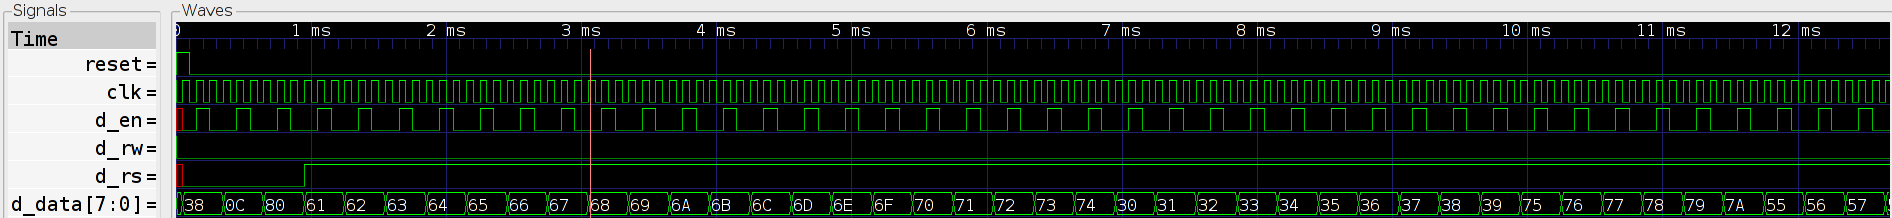
\includegraphics[width=\textwidth]{display_driver_timing_reset.png}
	\end{center}
	\caption{Simulated output of the display driver}
	\label{display_driver_waveform}
\end{figure}

\section{Time buffer}

\subsection{Overview}



\end{document}
